\label{sec:approx}

In this section, we present the main novel contribution of our paper
for approximating XADDs within a fixed error bound.  Since the point
of XADD approximation is to shrink its size, we refer to our method of
approximation as \emph{XADD compression} (\textsc{XADDComp}).

Following previous work on ADD compression~\cite{apricodd}, we note
that decision diagrams should be compressed from the bottom up ---
merging leaves causes simplifications to ripple upwards through a
decision diagram removing vacuous decisions and shrinking the decision
diagram.  For example, after merging leaves in
Figure~\ref{fig:stepfunfig}(a), we note that the only remaining
decision in \ref{fig:stepfunfig}(b) is $x < 3$.  Hence, we focus on a
leaf merging approach to \textsc{XADDComp}, which poses two questions:
(1) what leaves do we merge, and (2) how do we find the best
approximation of merged leaves?  We answer these two questions in the
following subsections.

%A novel method for approximating piecewise linear functions with
%bounded error. The goal of this algorithm is to reduce the number of
%partitions of a piecewise linear function represented in case
%form. This represents the ability to automatically identify and remove
%locally unimportant constraints, whose removal results in a small
%change in the represented function in exchange for a significant
%improvement in the efficiency of computations with these
%functions. XADDs already permit compactness by exploring variable and
%context independencies, so our approximate approach goes further to
%merge partitions as a form of removing dependencies that had little
%influence in the represented function.

%% NOTE: No paper uses all caps for section headings... it's like
%% yelling at the reader. :)
% !!! It is the UAI Style, as in the sample.tex !
%\subsection{SUCCESSIVE MERGING}

%%%%%%%%%%%%%%%%%%%%%%%%%%%%%%%%%%%%%%%%%%%%%%%%%%%%%%%%%%%%%%%%%%%%%%
%%                     Scott stopped editing here - and this has changed almost everything....
%%			I am glad that you have improved so many things, but it does seem bad that there %% 			were so many "mistakes",
%%%%%%%%%%%%%%%%%%%%%%%%%%%%%%%%%%%%%%%%%%%%%%%%%%%%%%%%%%%%%%%%%%%%%%

\subsection{Successive Leaf Merging}

A straightforward way of attempting to find the optimal way of merging leaves would require evaluation of the combinatorial possibilities of partitioning of all leaves and is hardly practical. A simpler, but more efficient approach is to repeatedly consider the simpler problem of merging just two leaves. In this case it seems reasonable to find the pair of leaves that incurs the smallest error upon merging and repeat this while any of the pairs can still be merged with the allowed error. Thus, our approximation algorithm, Alg.~\ref{alg:approx} uses a constructive strategy to obtain merging of arbitrary regions by successive pairwise merging of partitions. This idea is simple and is illustrated in figure~\ref{fig:steplining}. The bounded error property is guaranteed by storing the amount of error "used" in every merge and avoiding any merges that incur more error than the remaining allowed error on one of the nodes being currently merged.

\begin{figure}[!ht]
\centering
  \subfigure[Original] {
  	\begin{minipage}{.25\textwidth}
	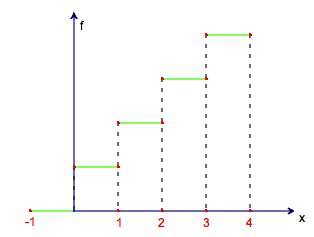
\includegraphics[width=\textwidth]{Figures/stepfun/succ1.png}
	\end{minipage}
	\begin{minipage}{.2\textwidth}
	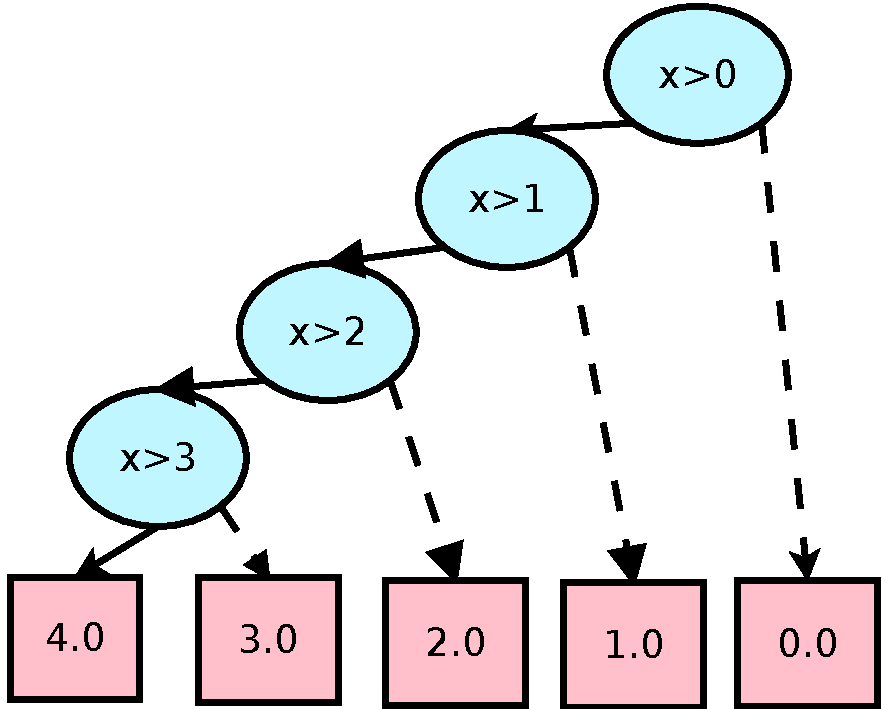
\includegraphics[width=\textwidth]{Figures/xadds/succ1.pdf}
	\end{minipage}
	\label{original}
  }
\subfigure[Step1] {
  	\begin{minipage}{.25\textwidth}
	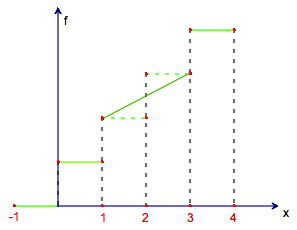
\includegraphics[width=\textwidth]{Figures/stepfun/succ2.png}
	\end{minipage}
	\begin{minipage}{.2\textwidth}
	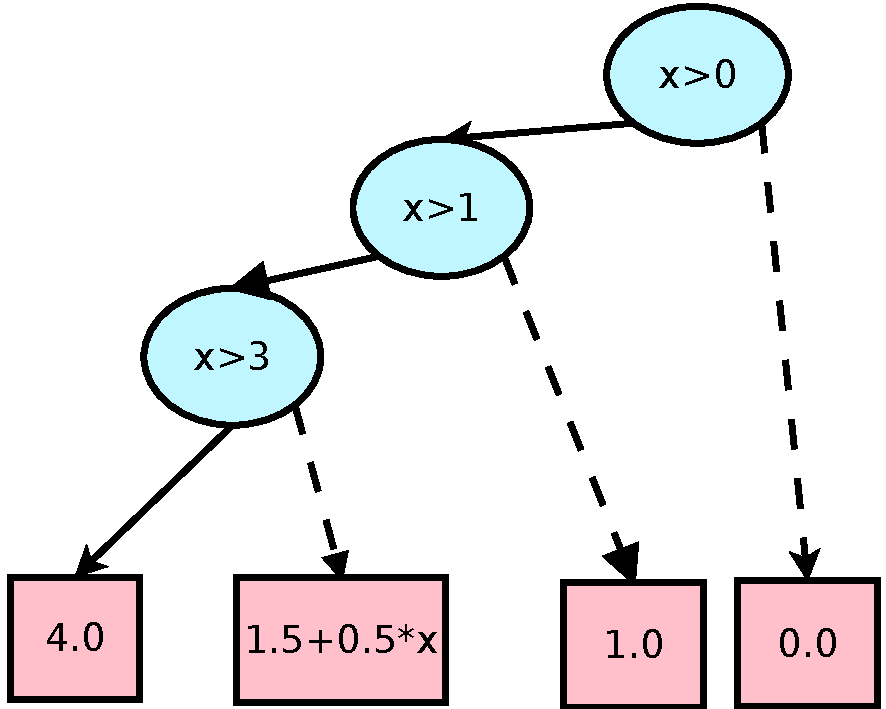
\includegraphics[width=\textwidth]{Figures/xadds/succ2.pdf}
	\end{minipage}
	\label{step1} 
}
\subfigure[Step2]{
  	\begin{minipage}{.25\textwidth}
	 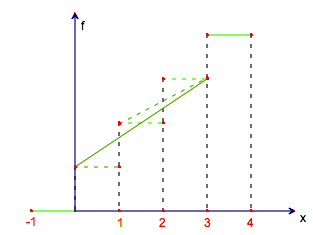
\includegraphics[width=\textwidth]{Figures/stepfun/succ3.png}
	\end{minipage}
	\begin{minipage}{.2\textwidth}
	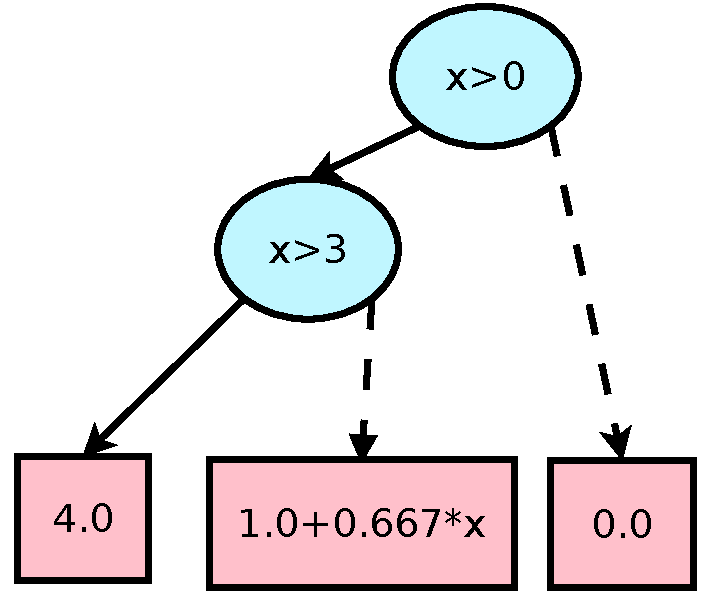
\includegraphics[width=\textwidth]{Figures/xadds/succ3.pdf}
	\end{minipage}
	 \label{step2}
}
\caption{ Approximation by successive pair merging}
 \label{fig:steplining}
\end{figure}

\incmargin{1.5em}
\linesnumbered
\begin{algorithm}[!ht]
\dontprintsemicolon
\KwIn{A piecewise linear function $V$, relative\_allow\_error}
\KwOut{Approximated version of $V$.}
$M \gets MaxValue(V)$
$allow\_error \gets M * relative\_allow\_error$
$OpenCases \gets getCases(V)$\;
\While{$OpenCases != \emptyset$} {
	$L_1 = OpenCases.pop()$\;
	$error = allow\_error$\;
	\For{$ L_2 \in OpenCase$}  { 
		$MergeResult = PairwiseCaseMax( L_1, L_2)$\;
		\If {$ MergeResult.error < error $} 
		{
			$error \gets error - MergeResult.error$\;
			$OpenCases.remove(L_2)$\;
			$ Remap(L_1, MergeResult.L^*) $\;
			$ Remap(L_2, MergeResult.L^*) $\;
			$ L_1 \gets MergeResult.L^* $\;
		}
	}
}
\Return{ApplyRemap(V)}\;
\caption{{\sc Approximate}: bounded approximation of piecewise linear function}
\label{alg:approx}
\end{algorithm}
\decmargin{1.5em}

\subsection{Pairwise Leaf Approximation}

We now focus on the pairwise case linear function approximation. The most important step in our solution to piecewise linear function approximation is the iterative linear program based algorithm for obtaining optimal, that is, max-error minimizing, case linear function to approximate any pair of case linear functions. In order to explain our algorithm more conveniently, we make the following consideration.

Since the continuous domain of a case linear function is independent of boolean variable decisions, they do not interfere with the constrained maximization of the linear functions and therefore don't affect the merging of case linear functions. Hence, for clarity, we will consider piecewise linear functions whose partitions are defined only with linear inequalities.

We can now define the optimal merging of case linear functions as an optimization problem. Formally, given two case linear functions $L_1 = ( f_1, \phi_1 )$ and $L_2 = ( f_2, \phi_2 )$, our goal is to determine the best linear case approximation of $L_1$ and $L_2$. As it must represent  $L_1$ and $L_2$, the solution must be defined in both regions, therefore of the form $L^* = (f^*,\phi_1 \lor  \phi_2)$. As a linear function $f$ over $\vec{x} \in \mathbb{R}^m$ is equivalent to a coefficient vector $\vec{c} \in \mathbb{R}^{m+1}$, we can define $\vec{c_1}$ and $\vec{c_2}$ as the coefficient vectors of $f_1$ and $f_2$, respectively. Searching for the optimal linear function $f^*$ can be restated as searching for optimal coefficients $\vec{c^*}$. Thus our optimization problem can be written as:
\begin{equation} \min_{\vec{c}} \max_{i} \max_{\vec{x} \in C(\phi_i)} \big( |(\vec{c} - \vec{c}_i)\cdot \vec{x}| \big)  \label{eq:optimglo} \end{equation}

Which is a piecewise saddle bilinear program, as the objective function is bilinear $\vec{c} \cdot \vec{x}$, there is maximization in $\vec{x}$ in piecewise linear regions $C(\phi_i)$ and minimization in $\vec{c}$. Defining a function to represent the error in each region, $Err_i$, this can be rewritten as:

\begin{equation} \min_{\vec{c}} \left[ \max \big( Err_1(\vec{c}), Err_2(\vec{c}) \big) \right] \label{eq:minc} \end{equation}
where
\begin{equation} Err_i(\vec{c}) = \max_{\vec{x_i}} \big(  | (\vec{c}-\vec{c_i}) \cdot \vec{x} |\big) \label{eq:errc} \end
{equation}
$$\text{s.t.} \hspace{1cm} \vec{x} \in C(\phi_i)$$

Note that the absolute values in~\ref{eq:errc} are equivalent to max of two linear functions, e.g. $\max_y (|g(y)|) = \max \big( \max_y g(y), \max_y -g(y) \big)$. Moreover, a maximization within a regions $C(\phi_i)$, is equivalent to the max of the maximization in all polytopes $Polyt(\theta_{ij})$ of $\phi_i$. With this, we can rewrite the error $Err_i$, as the maximum of a finite number maximizations of bilinear functions with linear constraints in $\vec{x}$:
{\footnotesize 
\vspace{-2mm}
\begin{equation} Err_i(\vec{c}) = \max_{j=1..n_i} \big( max ( err^+_{ij}(\vec{c}), err^-_{ij}(\vec{c}) ) \big) \label{eq:errcij} \end{equation}
\vspace{-5mm}

where, for $i=1,2$ and $j=1..n_i$
\vspace{-1mm}
\begin{equation} err^{\pm}_{ij}(\vec{c}) = \max_{\vec{x} \in Polyt(\theta_{ij})} \big( \pm(\vec{c} - \vec{c}_i)\cdot \vec{x} \big)  \label{eq:polymax} \end{equation}
\vspace{-2mm}
}

Now our optimization problem is clearly defined in a three stage optimization: (i) maximization within a polytope with the original continuous variables $\vec{x}$; (ii) discrete maximization of the between the polytopes; and (iii) minimization of this global max with the coefficients $\vec{c}$. It is illustrated in figure~\ref{fig:optim}.

\begin{equation} \min_{\vec{c}} \max_{i,j} \max_{\vec{x} \in Polyt(\theta_{ij})} \big( |(\vec{c} - \vec{c}_i)\cdot \vec{x}| \big)  \label{eq:optimglo} \end{equation}


\begin{figure}[h!t]
\center
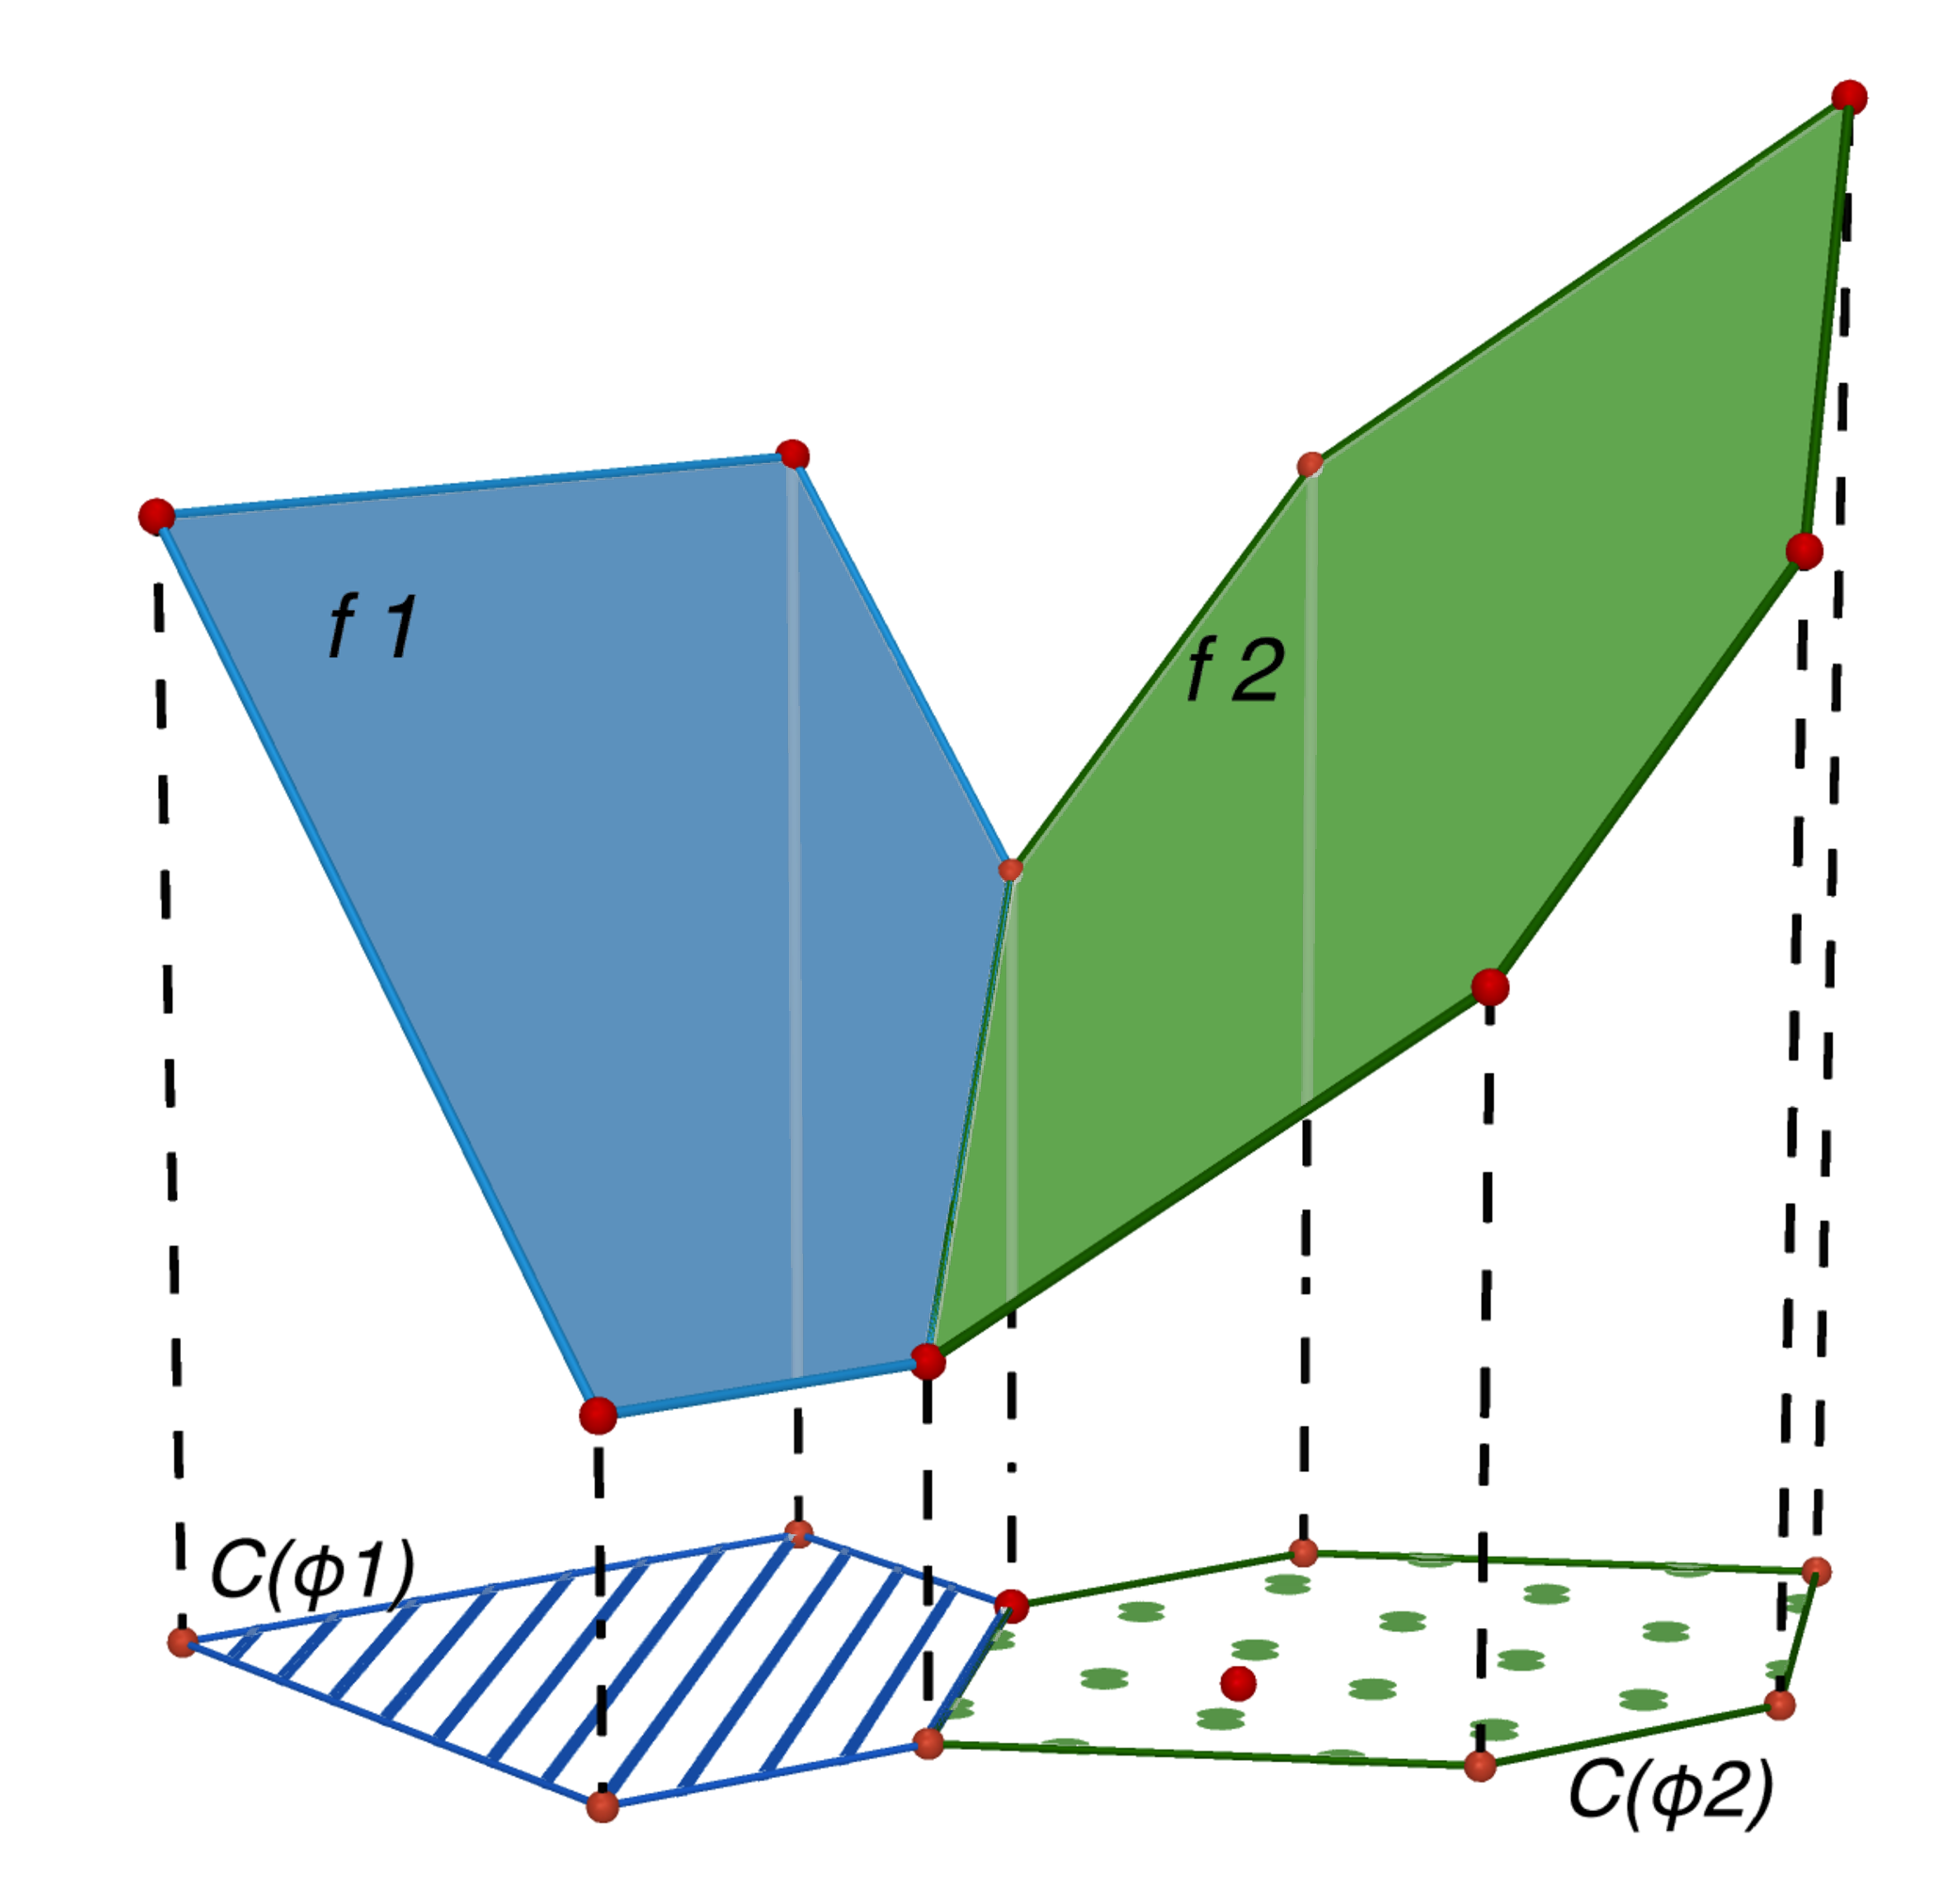
\includegraphics[trim = 2cm 0cm 2cm 0cm, height=0.25\textwidth,width=0.2\textwidth]{Figures/optimDiag/optdiagram1.pdf} 
\hspace{2mm}
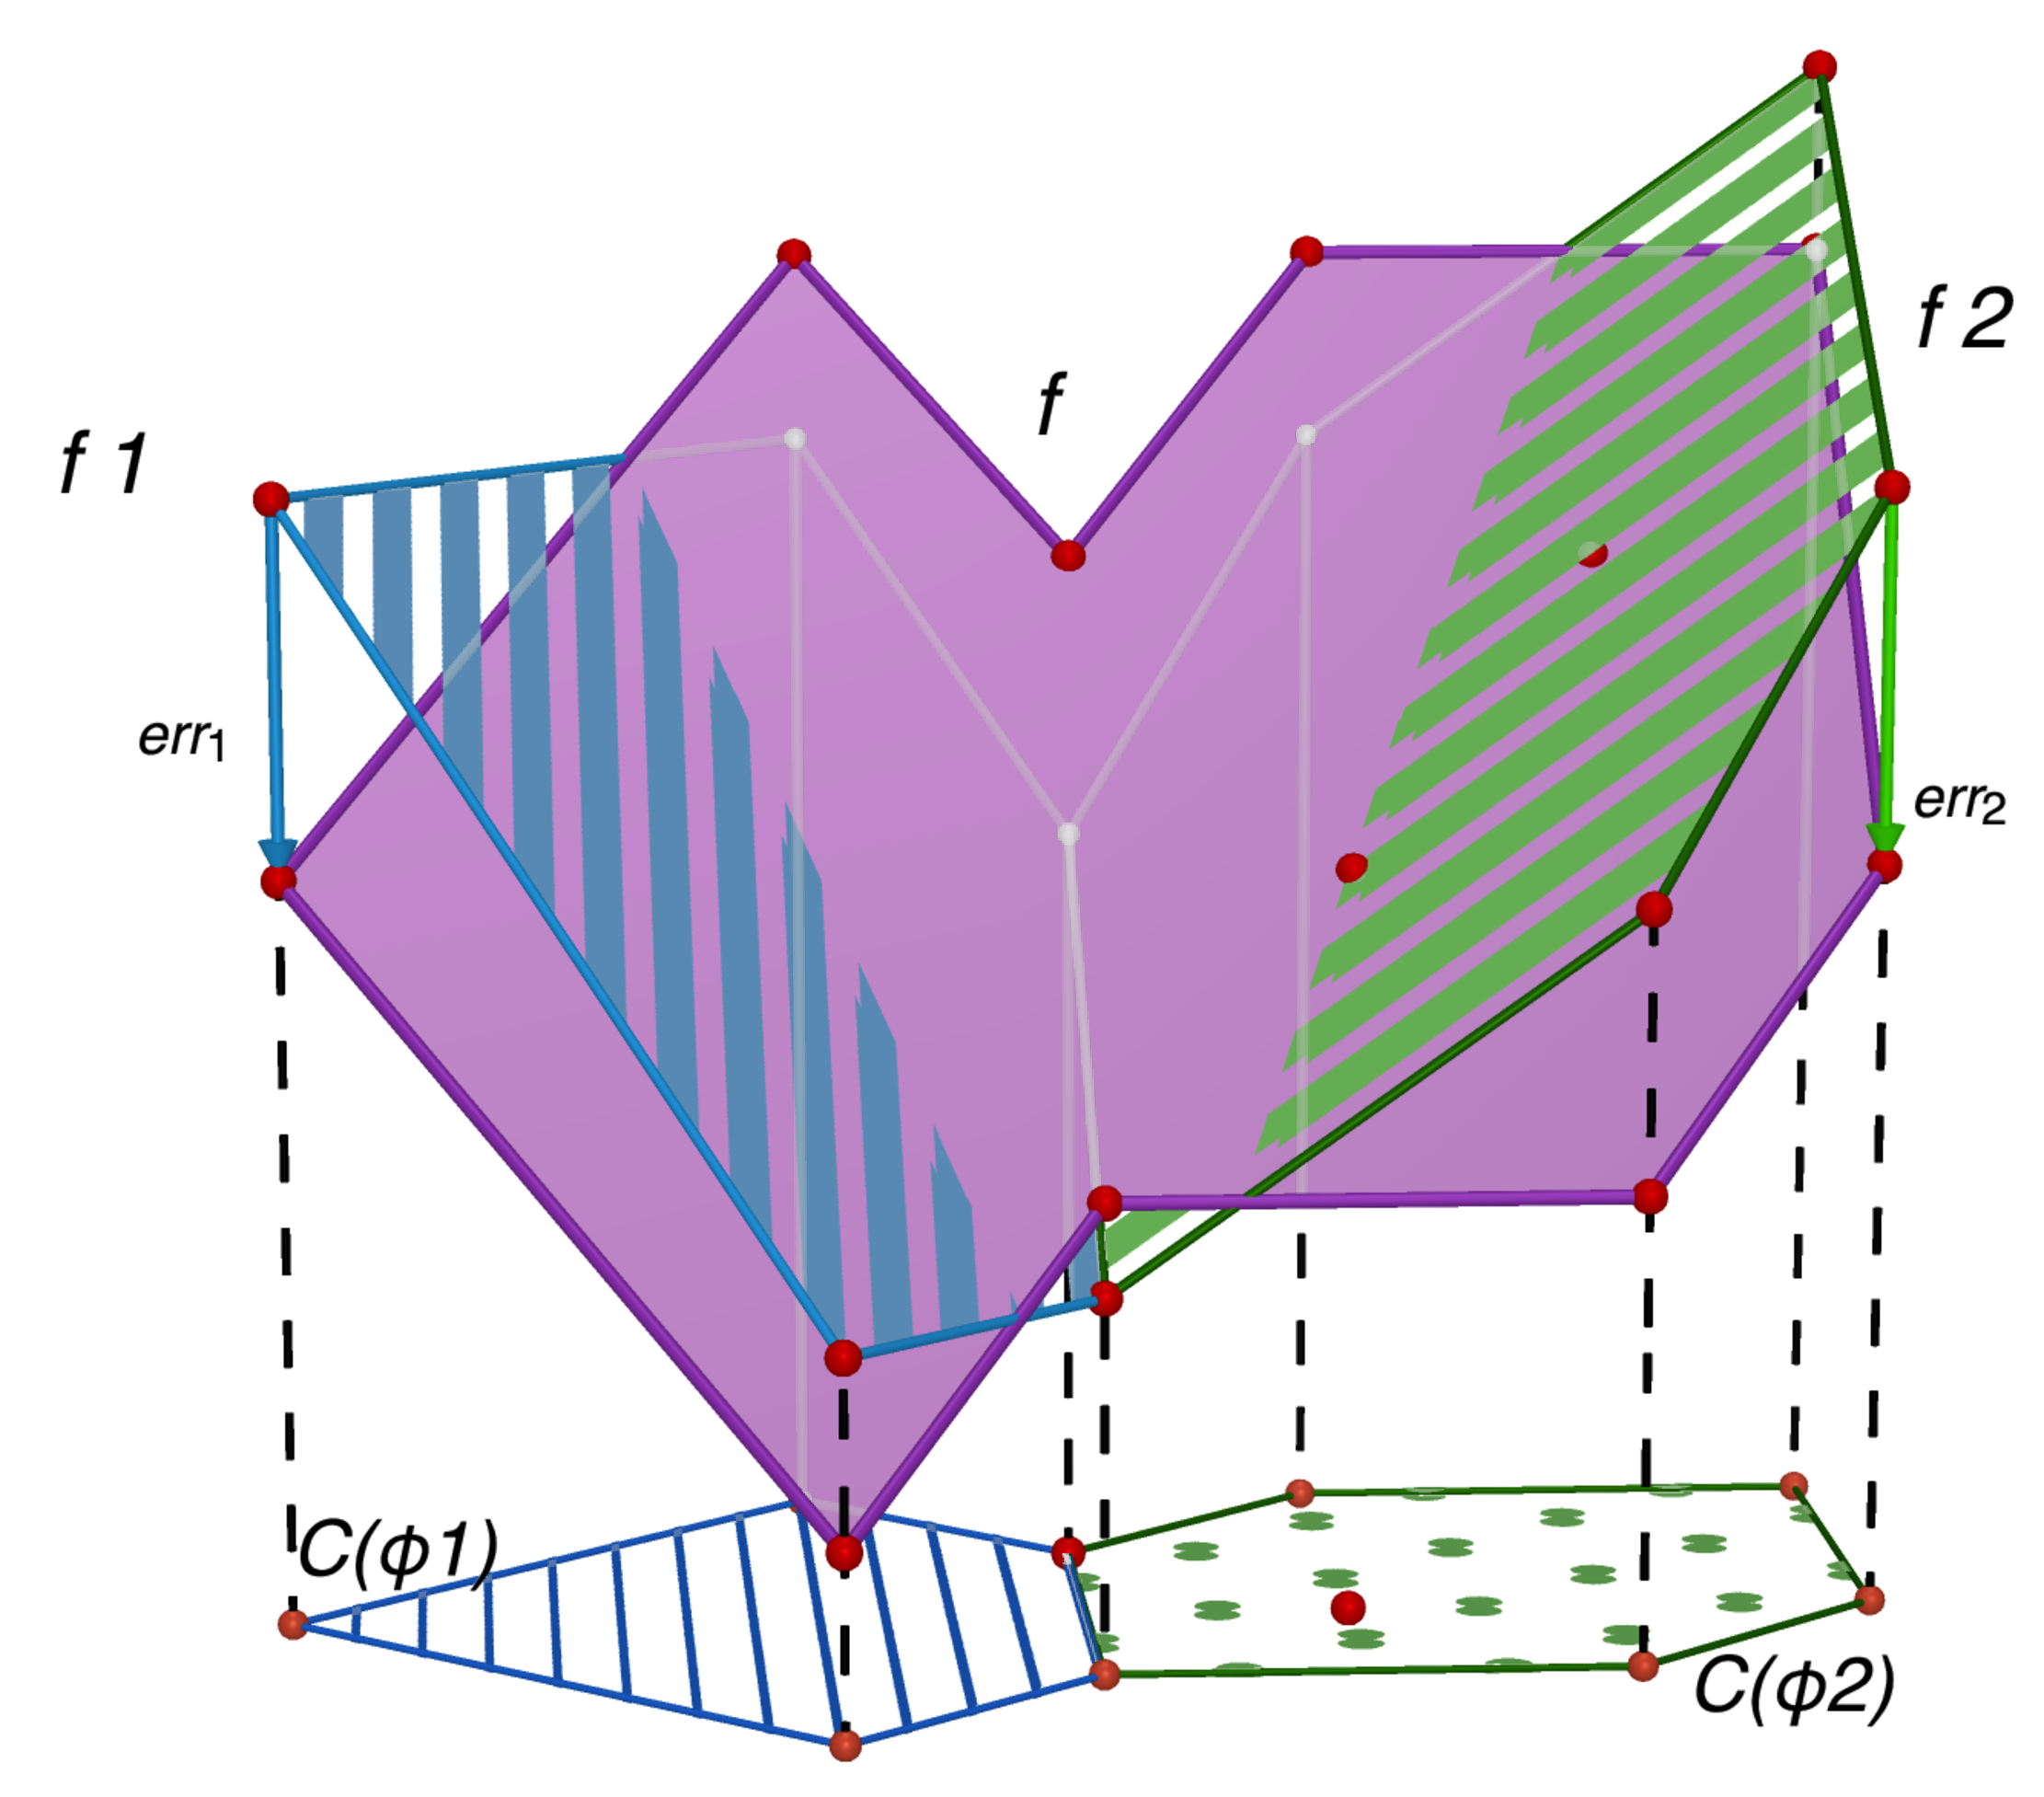
\includegraphics[trim = 2cm 0cm 2cm 0cm, height=0.25\textwidth,width=0.2\textwidth]{Figures/optimDiag/optdiagram2.pdf}
\caption{Illustration of the piecewise linear merging problem: \emph{(left)} the original linear functions in their regions; \emph{(right)} a linear approximation defined on the merged region.}
\label{fig:optim} 
\end{figure}


In order to solve this, we propose an iterative constraint generation based algorithm which we describe in the following. First, the algorithm will iterate between two phases, one for the maximization and one for the minimization.  Second, on each phase a relaxed problem will be solved using the result from the previous phase. Finally, when a phase gives the same solution twice, the algorithm has converged and a solution to the original problem was found.

In the maximization phase, related to Eq.~\ref{eq:polymax}, we will assume a fixed $\vec{c}$, and thus the maximization of the bilinear functions $\pm(\vec{c} - \vec{c}_i)\cdot \vec{x}$ for each polytope will be linear constrained linear objective problems, solved efficiently by a LP solver. The optimal values are maximum errors in each polytope, the maximum of which is an upper bound on the optimal approximation error, simply because this $\vec{c}$ is a valid function and if no other function gives a better approximation we can use it and the error is exactly the one we just obtained. More importantly, the vertices that reach these optimal values are the points of the polytope that maximize the bilinear function for this value of $\vec{c}$ and therefore are important points for the minimization phase. In fact, if the minimization can't reduce the error in these points, it can't change the maximal error, and thus has achieved the optimal solution. The maximal error points from each polytope are stored at every iteration through the maximization phase, $x^{+t}_{ij}$ and $x^{-t}_{ij}$ are the points found in the $t$-th maximization for the polytope $\theta_{ij}$. 

In the minimization phase, we will solve a relaxation of the problem in Eq.~\ref{eq:minc}, where in each linear constrained bilinear function $err^{\pm}_{ij}$ the maximal error in the polytope $\theta_{ij}$ is replaced by the greatest error from a finite set of points from polytope. More specifically, we only minimize the greatest of the error on points found in the maximization phase. This changes the piecewise bilinear problem into a linear program with the objective to be minimized is a new variable $Z$ that symbolizes the maximal error. There are linear constraints to encode that $Z$ must be greater than any of the errors on the points selected in the previous iterations. For all polytopes $\theta_{ij}$ and previous iterations $t$ the points selected are $x^{\pm t}_{ij}$ and the error at there points is $\tilde{err}_{ij}^{\pm t}(\vec{c})$.

$$ \tilde{err}_{ij}^{\pm t} (\vec{c}) = \big( \pm (\vec{c}_i - \vec{c})\cdot \vec{x}_{ij}^{\pm t} \big)$$
$$ \tilde{Err}(\vec{c}) =\max_{i,j,t} \big( \tilde{err}^{+t}_{ij} (\vec{c}), \tilde{err}^{-t}_{ij} (\vec{c}) \big)$$
And the optimization becomes:
$$min_{\vec{c}}\tilde{Err}({\vec{c}}) = min_{{\vec{c}},Z}  Z $$
s.t. 
$$
	\begin{array}{llll}
		Z & \geq & \tilde{err}_{ij}^{+t} (\vec{c}) & \mbox{for } i=1,2; j = 1..n_i; t=1..T\\
		Z & \geq & \tilde{err}_{ij}^{-t} (\vec{c}) & \mbox{for } i=1,2; j = 1..n_i; t=1..T\\
	\end{array}
$$
where $T$ is the current iteration.

This is now a linear problem in the coefficients $\vec{c}$ and $Z$. Solving this minimization yields a new solution $\vec{c}$ that minimizes the greatest error in all these points. As important points may still have not been considered this is a lower bound in the optimal approximation error. This can be seen by the following: $f$ may have to be modified to minimize the error in more points in the next iterations, but this can only lead to increasing the error in the points that were present in this iteration. This follows directly from the fact that adding more constraints cannot improve the optimal value of solution for a linear program.

The pseudocode for the algorithm just described is algorithm~\ref{alg:glo}. The algorithms ~\ref{alg:maxError} and ~\ref{alg:relaxApprox} encode, respectively, the maximization and the minimization phases. Both use an abstract call to a linear programming solver, $LP\_Solve($ max or min$, objective\_function, linear\_constraints)$ which returns the solution and optimal value for the linear program received.

\incmargin{1.5em}
\linesnumbered
\begin{algorithm}[!ht]
\dontprintsemicolon
\KwIn{Linear cases  $L_1 = ( f_1, \phi_1 )$, $L_2 = ( f_2, \phi_2 ).$}
\KwOut{ $(L^*, error)$ s.t. $L^*$ approximates $L_1$ and $L_2$.}
$f \gets 0$\;
$points \gets \emptyset$\;
$new\_points, error = MAX\_ERROR(f, L_1,L_2)$\;
\While{$new\_points \not \subset points$} {
	$points = points \cup new\_points$\;
	$f = BEST\_APPROX(f_1,f_2,points)$\;
	$new\_points, error = MAX\_ERROR(f, L_1,L_2)$\;}
\Return{$( (f, \phi_1 \lor \phi_2), error )$}\;
\caption{{\sc PairwiseCaseMax} finds the best case linear function}
\label{alg:glo}
\end{algorithm}
\decmargin{1.5em}

\incmargin{1.5em}
\linesnumbered
\begin{algorithm}[!ht]
\dontprintsemicolon
\KwIn{Case linear functions $L_1 = ( f_1, \phi_1 ), L_2 = ( f_2, \phi_2 )$ and function $f$ }
\KwOut{Set of points where the error is maximal for each polytope and the optimal $error$.}
$max\_points \gets \emptyset$\;
$error \gets NEG\_INF$\;
\For {$\theta_1 \in Poly(\phi1)$} {
	$sol^+, obj^+ \gets LP\_Solve(max _x, f-f_1,\theta_1) )$\;
	$sol^-, obj^- \gets LP\_Solve(max _x, f_1-f,\theta_1) )$\;
	$max\_points.add(sol^+,sol^-)$\; 	$error \gets max(error, obj^+, obj^-)$\; 
	}
\For {$\theta_2 \in Poly(\phi2)$} {
	$sol^+, obj^+ \gets LP\_Solve(max _x, f-f_2,\theta_2) )$\;
	$sol^-, obj^- \gets LP\_Solve(max _x, f_2-f,\theta_2) )$\;
	$max\_points.add(sol^+,sol^-)$\; 	$error \gets max(error, obj^+, obj^-)$\; 
	}\Return{$(max\_points, error)$}\;
\caption{{\sc MAX\_ERROR} finds the points of maximum error}
\label{alg:maxError}
\end{algorithm}
\decmargin{1.5em}

\incmargin{1.5em}
\linesnumbered
\begin{algorithm}[!ht]
\dontprintsemicolon
\KwIn{Linear cases $L_1 = ( f_1, \phi_1 ), L_2 = ( f_2, \phi_2 )$ and a set of $points$ where to find the best approximation for}
\KwOut{Best linear case approximation $f$.}
$constr \gets \emptyset$\;
\For {$p \in points$}{ 
	\If {$p \in \phi_1$}{
		$constr \gets constr \cup \{ (Z \geq (f - f_1) (p)), (Z \geq (f_1 - f) (p) )\} $}\;
	\If {$p \in \phi_2$}{
		$constr \gets constr \cup \{ (Z \geq (f - f_2) (p)), (Z \geq (f_2 - f) (p) )\} $}\;
}\;
$f \gets LP\_Solve(min_{f,Z}, Z, constr)$\;	
\Return{$f$}\;
\caption{{\sc BEST\_APPROX} finds the linear function minimizing errors a set of points}
\label{alg:relaxApprox}
\end{algorithm}
\decmargin{1.5em}

Finally, we prove some properties of the developed algorithm.

{\bf Theorem} {\it Algorithm~\ref{alg:glo} always terminates and produces the optimal solution for the optimization described in Eqs.~\ref{eq:minc},~\ref{eq:errcij},~\ref{eq:polymax}.} 

To prove the optimality of the solution obtained, we observe that at the beginning of the loop the algorithm always keeps an optimal approximation $f$ for all $points$ stored. Using this $f$ the $MAX\_ERROR$ routine computes new points that are the maximum error points for this $f$. If there are new points, these are added to the stored points and $BEST\_APPROX$ computes a new $f$ that minimizes in all stored points. As we return to the start of the loop we have a new optimal approximation. If there are no new points, this means that the current $f$ minimizes the error in the points that maximize its error therefore it minimizes the maximal error in all regions and is the optimal solution.  As the algorithm only terminates when there are no new points, and in this case the solution is optimal, if the algorithm terminates, its solution is optimal.
 Next we prove that the algorithm must terminate: First, the formulae $\phi$  are finite and define a finite number of polytopes. Second, for all polytopes defined, there is a finite number of inequalities and correspondingly a finite number of vertices. At each non terminal iteration at least one new polytope vertex must be added to the stored $points$ list, as there are finitely many vertices, the number of iterations must be finite, so the algorithm terminates.





